%!TEX root = Thesis.tex
\chapter{Implementation and Evaluation}
	The chapter contains practical part of the work, describing implementation of modules defined in the Chapter 4 within a convincing scenario. The prototype implements major aspects proposed in the concept, including following tiers:
	 \begin{itemize}
		\item \textbf{Client Tier} includes adaptive GUI with related libraries, modules for dynamic content updates and session management;
		\item \textbf{Application Tier} contains XMPP server with protocol extensions, ensuring appropriate interface for communication between tiers;
		\item \textbf{Data Tier} contains descriptional metadata of sensors and is responsible for streaming text, images or arbitary data provided by heterogeneous sources.
	\end{itemize}
	To make precise evaluation, system will use real data from temperature sensor which is provided by ACDSense project, together with TU Dresden, BTU Cottbus-Senftenberg and RWTH Aachen University. It is located in the room INF3084, Faculty of Computer Science, Chair of Computer Science.


\section{Implementation requirements}
\subsection{Programming language and libraries}
In order to maximize application compatibility, standard web-stack tools have been selected for this work: Javascript for frontend logic, HTML\footnote{HTML specification, \url{http://www.w3.org/wiki/HTML/Specifications}} for layout markup, CSS\footnote{CSS specification, \url{http://www.w3.org/Style/CSS/specs.en.html}} for block styling.

To select additional software tools responsible for css selectors, function chaining, event handlers, AJAX etc, a comprehensive comparison of libraries was made, including most popular web toolkits like jQuery\footnote{jQuery Javascript library, \url{http://jquery.com/}}, Dojo\footnote{Dojo documentation, \url{http://dojotoolkit.org/features/}}, Prototype\footnote{Prototype documentation, \url{http://prototypejs.org/}}, Yahoo User Interface(YUI) and ExtJS\footnote{ExtJS documentation,\url{http://docs.sencha.com/extjs/4.2.2/}}, as shown in the Table 5.1. 
\begin{table}[H]
\centering
\begin{tabular}{|L{3cm}|l|L{2cm}|l|L{2cm}|L{2cm}|}
\hline
Target 			& jQuery & Dojo & Prototype & YUI & ExtJS \\
\hline
\hline
License		& MIT & BSD \& AFL & MIT & BSD & GPL and Commercial \\
\hline
Size		& 32 kB & 41 kB & 46–278 kB & 31 kB & 84–502 kB \\
\hline
Dependencies		& JavaScript & JavaScript + HTML & JavaScript &  Javascript + HTML + CSS & JavaScript \\
\hline
Layout Grid		& yes & yes & yes & - & yes  \\
\hline
DOM wrapped		& yes & yes & yes & no & yes \\
\hline
Data retrieval formats		& XML, HTML & XML, HTML, CSV, ATOM & - & yes & XML  \\
\hline
Server push data retrieval		& yes & yes & - & via plugin & yes \\
\hline 		
Touch events		& with plugin & yes & yes & - & yes \\
\hline 
\end{tabular}
\caption[Comparison of JavaScript frameworks]{Comparison of JavaScript frameworks}
\label{tab:JS_frameworks}
\end{table}
Also the most important part is browser support which is presented in the Table 5.2 . jQuery\footnote{jQuery browser support, \url{http://jquery.com/browser-support/}}, Dojo\footnote{Dojo browser support,\url{http://livedocs.dojotoolkit.org/releasenotes/1.4}}, Prototype\footnote{Prototype browser support, \url{http://prototypejs.org/doc/latest/Prototype/Browser/index.html}}, YUI\footnote{YUI browser support, \url{http://yuilibrary.com/yui/environments/}}, ExtJS\footnote{ExtJS browser support, \url{http://www.sencha.com/products/extjs/}}.

\begin{table}[H]
\centering
\begin{tabular}{|r|l|l|l|l|l|}
\hline
Target 			& jQuery & Dojo & Prototype & YUI & ExtJS \\
\hline
\hline
Chrome		& 1+ & 3 & 1+ & - & 10+ \\
\hline
Opera		& 9+ & 10.50+ & 9.25+ & 10.0+ & 11+ \\
\hline
Safari		& 3+ & 4 & 2.0.4+ & 4.0 & 4+ \\
\hline
Mozilla Firefox		& 2+ & 3+ & 1.5+ & 3+ & 3.6+ \\
\hline
Internet Explorer		& 6+ & 6+ & 6+ & 6+ & 6+ \\
\hline
\end{tabular}
\caption[Browser Support]{Browser Support}
\end{table}


 Considering aforesaid evaluation, jQuery library has been selected as a main Javascript dependency. The goal of such software components selection is to make resulting code more short, readable, and easier to support for other developers.

\subsection{Frontent Frameworks}
\subsubsection{Integrating CSS toolkit}
Twitter Bootstrap was selected as one of the most popular and widely used css frameworks nowadays, offering basic style and usability components for web pages, such as responsive CSS grid, adaptive class mixins, various widgets, etc. 

It consists of four main modules:
\begin{enumerate}
\item Scaffolding – global styles, responsive 12-column grids and layouts. Has some expressive features like tablets and mobile grids which maintain the grid column structure instead of collapsing the grid columns into individual rows when the viewport is below 768 or 480 pixels wide.
\item Base CSS – this includes fundamental HTML elements like tables, forms, buttons, and images, styled and enhanced with extensible classes.
\item Components – collection of reusable components like dropdowns, button groups, navigation controls (tabs, pills, lists, breadcrumbs, pagination), thumbnails, progress bars, media objects, and more.
\item JavaScript – jQuery plugins which bring the above components to life, and adding transitions, modals, tool tips, popovers, scrollspy, carousel, typeahead, affix navigation, and more. 
\end{enumerate}

It was decided to use first three modules for GUI development, maximally reducing Javascript dependencies. All animations, appearence, and dynamic adaptivity was done by using special tags, anchors and classes.

Examples of used modules are shown on a screenshots in the section \ref{section:use-case-scenario}. It contains buttons, navigation tabs bar, log in form, search field, 4/3/2-columns  grid layout, modals, tooltips and carousel for previews.

\subsubsection{Integrating JavaScript MVC}
As mentioned in the section \ref{section:web-frontend}, it is important to implement the system in a loosely-coupled way. Visualization, user management, content retrieving and data aggregation modules have to be separated and accessable through strictly defined interfaces.

In order to structure the code and enforce module decoupling, AngularJS\footnote{AngularJS,\url{http://angularjs.org/}} framework was selected. It assists running single-page application with a goal to augment it with model–view–controller (MVC) capability, making development, testing and support simpler.

Angular.js parces HTML that contains additional custom tag attributes; it then obeys the directives in those custom attributes, and binds input or output parts of the page to a model represented by standard JavaScript variables. The values of those JavaScript variables can be manually set, or retrieved from static or dynamic JSON resources\cite{ wiki:angular}. AngularJS is a toolset for building the framework most suited to application development. It is extensible and works well with other libraries such as jQuery. Every feature can be modified or replaced to suit unique development workflow and feature needs.

The framework adapts and extends traditional HTML to better serve dynamic content through two-way data-binding (Figure \ref{img:data-binding}) that allows automatic synchronization of models and views. As a result, AngularJS deemphasizes DOM manipulation and improves testability.

    \begin{figure}[!ht]
	\centering
	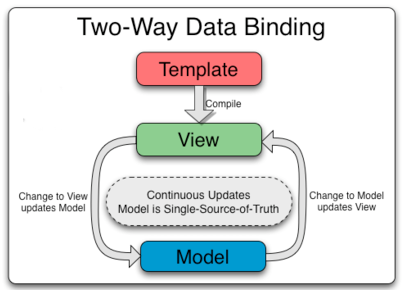
\includegraphics[scale=0.8]{images/2wayBinding.png}   
	\caption[Two-way data binding]{Two-way data binding\footnote{Angular JS Two-Way Data Binding,\url{http://docs.angularjs.org/guide/databinding}}}
	\label{img:data-binding}
	\end{figure}

\emph{Design goals}
\newline
Decouple DOM manipulation from application logic. This improves the testability of the code. Decouple the client side of an application from the server side. This allows development work to progress in parallel, and allows for reuse of both sides.	Angular follows the MVC pattern of software engineering and encourages loose coupling between presentation, data, and logic components. Using dependency injection, Angular brings traditional server-side services, such as view-dependent controllers, to client-side web applications. Consequently, much of the overheads on the backend is reduced, leading to much lighter web applications.

\emph{Two-way data binding}
\newline
AngularJS two-way data binding is a most notable feature and reduces the amount of code written by relieving the server backend from templating responsibilities. Instead, templates are rendered in plain HTML according to data contained in a scope defined in the model. The \$scope service in Angular detects changes to the model section and modifies HTML expressions in the view via a controller. Likewise, any alterations to the view are reflected in the model. This circumvents the need to actively manipulate the DOM and encourages bootstrapping and rapid prototyping of web applications.

The way Angular templates works is different, as illustrated on the Figure \ref{img:tmv}. They are different because first the template (which is the uncompiled HTML along with any additional markup or directives) is compiled on the browser, and second, the compilation step produces a live view. Any changes to the view are immediately reflected in the model, and any changes in the model are propagated to the view. This makes the model always the single source for the application state, simplifying the programming model for the developer. View is therefore an instant projection of a model.

    \begin{figure}[!ht]
	\centering
	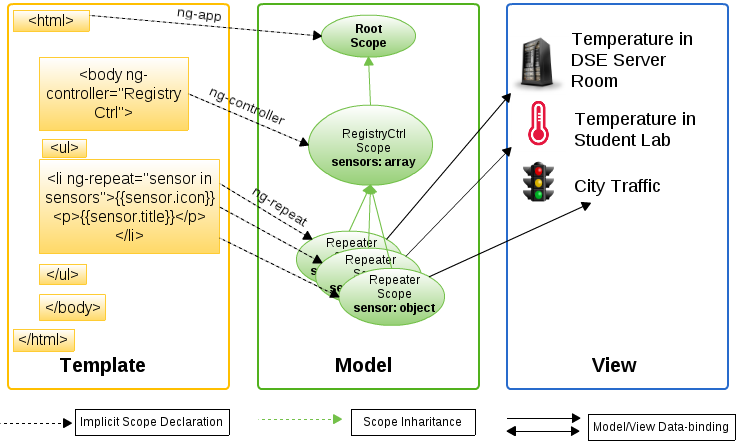
\includegraphics[scale=0.6]{images/3wayBinding.png}   
	\caption[Template Model View]{Template Model View} 
	\label{img:tmv}
	\end{figure}
    
Because the view is just a projection of the model, the controller is completely separated from the view and unaware of it. As shown on the figure above, the resulting view can be applied to every data available on a backend. Model handler automaticaly generates a view for every new sensor. No need to change code or add new id and dependent handlers, variables, channels. 

The template declaire the structure of what have to be shown on user view. Model repeats to generate the same view of every sensor in the list, which is coming from a controller as parameter {{sensor}} with possible attributes {{sensor.icon}} and {{sensor.titel}}, till the list of registered sensors will be finished.

The code of such flow is shown on the Listing~\ref{angular_template}.

	\begin{lstlisting}[label=angular_template,caption=Template registry.html]
<div id="sensor_list">
    <div class="grid-sizer"></div>
    <div class="masonry-brick sensor-wrapper" id="{{sensor.id}}" ng-repeat="sensor in sensors | filter:{title: query}">
        <div class="sensor" ng-controller="RegistryCtrl" ng-click="open()">
            <div class="icon">
                <img class="img-responsive" ng-src="{{sensor.icon}}">
                <h4>{{sensor.title}}</h4>
                <span class="label label-success" ng-show="user.check_subscribe(sensor.id)">Subscribed</span>
            </div>
            <div ng-show="sensor.picture">
                <img class="img-responsive" ng-src="{{sensor.picture}}">
            </div>
            <span class="description">{{sensor.description}}</span>
        </div>
    </div>
</div>
    \end{lstlisting}

Model is explicitly integrated to the HTML by using directives: ng-repeat, ng-src, ng-click and sensor prototype attributes {{sensor.*}}, as shown on the listing~\ref{angular_template}. Next, listing~\ref{angular_controller} shows the basic implementation of ``RegistryCtrl'' controller.

	\begin{lstlisting}[language=java,label=angular_controller,caption=Registry Controller]
var sensdash_controllers = angular.module("sensdash.controllers", []);

sensdash_controllers.controller("RegistryCtrl", ["$scope", "Registry", "User",
    function ($scope, Registry, User) {
        Registry.load().then(function(sensors){
            $scope.sensors = sensors;
        });
        $scope.user = User;
    }]);
    \end{lstlisting}


\subsection{XMPP support}

\subsubsection{Message broadcasting protocol}
In scope of this Master Thesis some limited conferencing functionality is required to broadcast messages from sensors to users. This functionality is partially covered in XMPP extensions. Two main extensions: MUC and PubSub will be described next, followed by decision of protocol support.

\textbf{XEP-0045: Multi-User Chat}
\newline
Multi-User Chat (MUC), is a standard XMPP conference protocol, supporting features like invitations, message presence, room moderation and administration, and specialized room types\footnote{XEP0045, \url{http://xmpp.org/extensions/xep-0045.html}}.

Each room is identified as a ``room JID'' <room@service> (e.g. <sensor@conference.tu-dresden.de>), where ``room'' is the name of the room and ``service'' is the hostname at which the multi-user chat service is running. Each occupant in a room is identified by ``occupant JID'' <room@service/nick>, where ``nick'' is the room nickname of the occupant as specified on entering the room or subsequently changed during the occupant's visit. A user enters a room (i.e. becomes an occupant) by sending directed presence to <room@service/nick>. An occupant can change the room nickname and availability status within the room by sending presence information to <room@service/newnick>. Messages sent within multi-user chat rooms are of a special type``groupchat'' and are addressed to the room itself (room@service), then reflected to all occupants. An occupant exits a room by sending presence of type ``unavailable'' to its current <room@service/nick>.

The MUC conference has next structure(Figure~\ref{img:muc-architecture}):
	\begin{figure}[!ht]
		\centering
		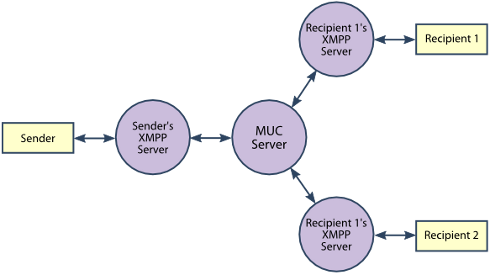
\includegraphics[scale=0.8]{images/MUC.png}
		\caption[MUC]{MUC System structure}
		\label{img:muc-architecture}                    
	\end{figure}

Group chat is provided as a service, usually having own domain. Each room on the group chat service gets its own address, which looks like a JID. Rooms can have access controls, moderators, administrators, and automatic logging and archival of the group communications.

\emph{Entering and Leaving a Room}
\newline
Joining and leaving a room is done using <presence> stanzas. Users can join a group chat room by sending available presence to the room. Similarly, to leave, unavailable presence is sent to the room.

If a user wants to join the group chat room with the Temperature sensor, they will both need to send directed presence to their desired identity in the room temperature@chat.sensor.lit. Their stanzas are shown in the Listing~\ref{code:stanzas_muc}:
\begin{lstlisting}[label=code:stanzas_muc,caption=Stanzas Format for MUC]
<presence to="temperature@chat.sensor.lit/sensor"
          from="sensor@example.lit/sensor">
    <x xmlns="http://jabber.org/protocol/muc"/>
</presence>
\end{lstlisting}

Once they have joined the room, the group chat service will broadcast all the other participants' presence statuses to them. After all the other participants’ presence stanzas are sent, the server concludes the presence broadcast by sending the arriving participant’s presence to everyone, including the new arrival. Thus, when a new participant sees their own presence broadcast back to them, they know they have fully joined the room.

The room sends the affiliations and roles of each participant along with their presence. Sensor's own presence broadcast also includes a status code of 110, which signals that this presence refers to the sensor itself. Just as with presence updates from sensor's roster, sensor will also receive presence updates from the room as people leave and new people join on the listing~\ref{code:muc_affiliation}.
\begin{lstlisting}[label=code:muc_affiliation,caption=Server Presence Notification]
<presence to="sensor@example.lit/sensor"
          from="temperature@chat.sensor.lit/sensor">
  <x xmlns="http://jabber.org/protocol/muc">
      <item affiliation="member" role="participant"/>
      <status code="110"/>
  </x>
</presence>
\end{lstlisting}

\emph{Creating Rooms}
\newline
Creating rooms is accomplished in the same manner as joining a room. Assuming the service allows the user to create new rooms, sending directed presence to the desired room JID of the new room will cause the room to be created and the user to be set as the room’s owner. On the Listing~\ref{code:room_creation}, sensor creates a new room for the News feed.

	\begin{lstlisting}[label=code:room_creation,caption=MUC Room Creation]
<presence to="chatter@chat.news.lit/sensor"
          from="sensor@news.lit/drawing_room">
    <x xmlns="http://jabber.org/protocol/muc"/>
</presence>
	\end{lstlisting}

The chat.news.lit service responds with the presence broadcast for the room’s new and only occupant.
Sensor has the owner affiliation and the moderator role. These attributes give the sensor special permissions within the room. More comprehensive information about roles, affiliations, erros and etc can be found in documentation \cite{XMPPbook}.

\textbf{XEP-0060: Publish-Subscribe}
\newline
Publish-subscribe is another conference XMPP extension\footnote{XEP-0060: Publish-Subscribe, \url{http://xmpp.org/extensions/xep-0060.html}} that provides a framework for a wide variety of applications, including news feeds, content syndication, extended presence, geolocation, trading systems, workflow systems, and any other application that requires event notifications (image~\ref{img:basic-pubsub}.

\begin{figure}[!ht]
    \centering
    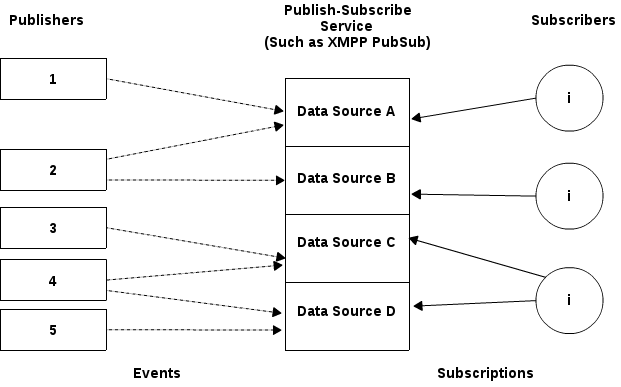
\includegraphics[scale=0.5]{images/XEP0060.png}   
    \caption[General Event Subscription]{General Event Subscription}  
    \label{img:basic-pubsub}                    
\end{figure}

There is a channel of communication, subscribers who are interested in data sent on that channel, and publishers who can send data across the channel. The first thing an application must do for a presenter is to create a channel to publish information. In XMPP pubsub these channels are called \emph{nodes}. The protocol enables XMPP entities to create nodes (services) at a pubsub service and publish information at those nodes; an event notification (with or without payload) is then broadcasted to all entities that have subscribed to the node. Pubsub therefore adheres to the classic Observer design pattern.

	\textbf{Creating a Node}
	\newline
	A pubsub node is created by sending an IQ-set stanza to the pubsub service, as shown in the listing~\ref{code:node_creation}, where User1 creates node ``sensor\_data'' within ``pubsub.sensor1.lit'' XMPP host server.
		\begin{lstlisting}[label=code:node_creation,caption=PubSub Node Creation]
	<iq to="pubsub.sensor1.lit"
	    from="user_1@sensor1.lit/sensor_registry"
	    type="set"
	    id="create1">
	  <pubsub xmlns="http://jabber.org/protocol/pubsub">
	      <create node="sensor_data"/>
	  </pubsub>
	</iq>
		\end{lstlisting}
	Most actions on pubsub nodes will look very similar to this one, the difference between MUC and PubSub stanzas is the <pubsub> element. Pubsub nodes and their configuration are necessary and useful, but they don't do much by themselves. The real value of pubsub nodes is in the events that are published to them and broadcast to subscribers. Anything can be included in a pubsub event. The pubsub service doesn’t know or care what is inside the event; it simply broadcasts this data to a node’s subscribers.

\emph{Retrieving Item}
\newline
User2 just subscribed to user1's sensor\_data node, and has missed his earlier event broadcasts.  User1 configured his node to persist items and anyone can query his node for the most recently published items. In listing~\ref{code:last-5-items}, user2 requests the last five items by sending an IQ-get stanza to the node with the <items>:
\begin{lstlisting}[label=code:last-5-items,caption=PubSub: requesting last 5 items from history]
<iq from="user2@longbourn.lit/outside"
    to="pubsub.sensor1.lit"
    type="get"
    id="items1">
  <pubsub xmlns="http://jabber.org/protocol/pubsub">
    <items node="sensor_data" max_items="5"/>
  </pubsub>
</iq>
\end{lstlisting}
The <items> element contains a node attribute just like the other actions. User2 has also set the max\_items attribute to 5 because he is only interested in the recent history. If he had omitted max\_items, the server would interpret it as a request to send all the historical data it has been configured to keep. If he had set max\_items to 500, which is much larger than the configured maximum for the node, the server would have sent as many as were available.

\emph{PubSub Data Flow}
\newline
Figure \ref{img:pub_sub} shows the process flow of how and when a client can subscribe/retrieve data from a publisher of service through the XMPP PubSub approach. The first thing the DataSource 1 and 2 must do for a would-be presenter is to create a channel for them to publish data - nodes. Once a node is created and configured, Publishers can start send data. Once these events are published, pubsub takes over and makes sure that they get delivered to the subscribed users. In case Publishers want to get a list of their subscribers, it can be retrieved from the pubsub node so that it can present this data to them. If Publisher will become offline its <presence> will be changed automatically to ``unavailable'' and next time, becoming online and sending new data, all subscribers will receive this information immediately.
    \begin{figure}[!ht]
    \centering
    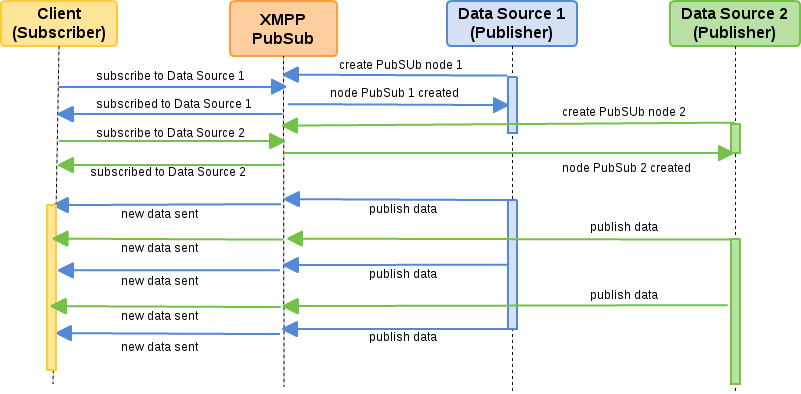
\includegraphics[scale=0.7]{images/PubSub.png}   
    \caption[Service PubSub]{Service PubSub}
    \label{img:pub_sub}                           
    \end{figure}
	    
\textbf{Comparison and Decision}
\newline
After reviewing possible ways to power message broadcasting mechanism, it is required to select the most appropriate one for implementation and support. A quick recap of muc/pubsub advantages and disadvantages is shown in table~\ref{tab:muc_vs_pubsub}.

\begin{table}[H]
	\centering
	\begin{tabular}{|L{0.5cm}|L{7.5cm}|L{7.5cm}|}
	\hline
	\textbf{}		& \textbf{Publish-Subscribe} & \textbf{Multi-User Chat} \\
	\hline
	\hline 
	\rot{\textbf{Advantages}}	
	&  \begin{itemize}
		\item Pubsub extension is generic, assuming nothing about the subscribers.
		\item Pubsub nodes and subscriptions are arranged in a tree-based hierarchy.
		\item Events can be published as notifications or as full payloads, and the subscriber can choose which is most appropriate.
		\item Retrieval of the publishing history is built in and fine grained.
		\item The subscriber has more fine grained control over the delivery destination. 
		\end{itemize}
	& \begin{itemize}
		\item MUC is optimized for chat-related use cases and builds on huge experience of previous chat systems, e.g. IRC.
		\item Presence handling is built in to MUC at a low level.
		\item Common moderation, administration and privelege features are supported.
		\item MUC has many implementations, both of clients and of servers.
		\item MUC allows for multiple levels of anonymity to be used as well as private communication.
		\end{itemize}\\
	\hline
	\rot{\textbf{Disadvantages}}
	&  \begin{itemize}
		\item By being generic, Pubsub is not optimized for specialized cases.
		\item Support for Pubsub features varies in quality and depth, e.g. no tools for node creation and configuration.
		\item No special handling of presence built in. 
		\item Tooling for pubsub node creation and configuration is lacking. 
		\item No built-in mechanism for subscribers to interact or find each other. 
		\end{itemize}
	& \begin{itemize}
		\item It is possible to have bots as room occupants, but the experience is designed for human consumption. 
		\item There is no way to organize chat rooms except as a flat hierarchy.
		\item There is no way to share configurations or participation across collections of rooms.
		\item Unlike pubsub, MUC implementations have a lot of edge cases in order to be user friendly and robust.
		\end{itemize}\\
	\hline
	\end{tabular}
	\caption[Pubsub and MUC comparison]{Pubsub and MUC comparison}
	\label{tab:muc_vs_pubsub}
	\end{table}

Although both approaches are very similar, each one has own set of strength and weaknesses. MUC implementation would ensure support of many existing systems, while having Pubsub would be more future-oriented. Therefore, it was decided to fully cover MUC extension, but also include a basic Pubsub integration, so that both systems can work in parralel if needed.

\subsubsection{XMPP connection with JavaScript}
In the web-application case, a connection to XMPP server can be only established through HTTP layer. This can be achieved by usnig Bidirectional-streams Over Synchronous HTTP (BOSH). Essentially, BOSH helps an HTTP client to establish a new XMPP session, then transports messages back and forth over HTTP wrapped in a special <body> element. It also provides some security features to make sure that XMPP sessions cannot be easily hijacked. The DataStream Manager communicates with the XMPP server as a normal client. In this way, an HTTP application can control a real XMPP session. Because of the efficiency and low latency afforded by the long polling technique, the end result competes with native connections.

Web applications are cross-platform, easily deployable, and come with a large user base already familiar with them. Web technologies rely on HTML, and it is usually the case that tools for manipulating HTML are also compatible with XML, making a good basis for work with XMPP stanzas. In order to implement web-based client-side application supporting XMPP streams Strophe.js\footnote{Strophe.js an XMPP library for JavaScript, MIT licensed, \url{http://strophe.im/strophejs/}} library was used.

\textbf{Strophe.js} is a library that will be used for invoking the XMPP protocol from a web-browser. While most of XMPP libraries are focused on chat-based applications, Strophe.js can to also power real-time games, notification systems and search engines, etc. It is production-ready since 2009, and therefore well tested, documented, and easy to extend. It uses BOSH, a standard binding of XMPP to HTTP using long polling.


\section{Interface Implementation}
	General architecture, as desined in the concept chaper, is shown on image~\ref{img:interfaces}
	\begin{figure}[!ht]
		\centering
		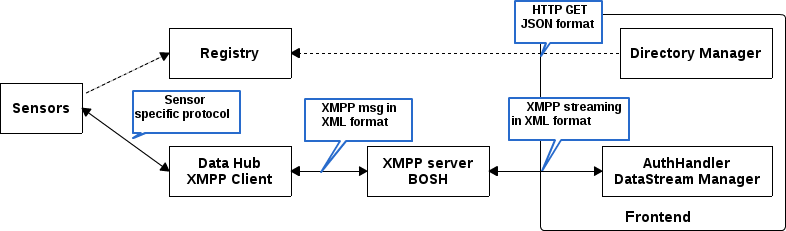
\includegraphics[scale=0.6]{images/XMPPflow.png}   
		\caption[System Interfaces]{System Interfaces}
        \label{img:interfaces}                      
		\end{figure}

	 According to it, frontend application has to implement two main interfaces:
	 \begin{enumerate}
	 \item Registry -- Directory Manager
	 \item XMPP/BOSH Server -- DataStream Manager and AuthHandler 
	 \end{enumerate}

	 Implementation of aforesaid interfaces and related modules will be described next.

\subsection{Directory Manager}
Directory Management module is responsible for querying registries and forming a list of available sensors along with metadata, such as availability and access information, SLA with expiration details, list of access endpoints etc.

As stated in the concept, in order to provide this data, Registries implement a simple Web-API, responding to GET requests with JSON list of available sensors. Since a user might have an unlimited number of registries, it is important to reduce his waiting time, so that a relation between amount of Web-API end-points and total loading time would not grow linearly.

A straightforward way to address the this issue is to query user Registries in parallel, making maximal loading time qeual to loading time of the slowest Registy. To accomplish this, the asynchronous Javascript nature will be used, combined with extension that implements defer/promise pattern: ``q-object'', provided by Angular.js.

The purpose of this deferred object is to expose the associated Promise instance as well as APIs that can be used for signaling the successful or unsuccessful completion and the status of the task. The q-object advantage over traditional callback approach is that the promise API allows for composition, in particular serial or parallel joining of promises.

The implementation of Directory Manager service, responsible for parallel querying of registries is shown on listing~\ref{code:q-object}. It is using http service requests combined into a single q-object, returned as a promice.  

    \begin{lstlisting}[language=java,label=code:q-object,caption=Parallel requests to Registies combinied in q-object]
	var sensdash_services = angular.module('sensdash.services', ['ngResource']);

	sensdash_services.factory("Registry", ["$http", "$q", "User", function ($http, $q, User) {
	    var registry = {
	        load: function () {
	            var requests = [];
	            var all_registries = User.registries.concat(Config.REGISTRIES);
	            for (var i = 0; i < all_registries.length; i++) {
	                requests.push($http.get(all_registries[i]));
	            }
	            var q = $q.all(requests);
	            var flat_list = q.then(function (result) {
	                var list = [];
	                for (var i = 0; i < result.length; i++) {
	                    list = list.concat(result[i].data);
	                }
	                return list;
	            });
	            return flat_list;
	        }
	    }
	    return registry;
	}])
    \end{lstlisting}

This way, controllers that require combined registry data will receive a promise object, resolved upon completion of all parallel HTTP requests.

\subsection{DataStream Manager}
A DataStream Manager is responsible for maintaineing an XMPP connection and provides access to it via HTTP long polling technique. This connection is going to be used for sending and receiving XMPP messages (stanzas) over XMPP stream. Stanzas will be regarded as a basic information block sent from Sensor to User, or from User to Data Hub.

Before any stanzas are sent, an XMPP stream is necessary. Before an XMPP stream can exist, a connection must be made to an XMPP server. Typically clients and servers utilize the domain name system (DNS) to resolve a server's domain name into an address they can connect to.

In the presented web application XMPP connections will be managed through the Connection object, implemented by Strophe library. DataStream Manager includes a pool of BOSH connection managers that require HTTP-bind URL to establish connections. Major XMPP servers come with support for BOSH built in, and they typically expose HTTP-bind service at http://example.com:5280/http-bind or http://example.com:5280/xmpp-httpbind.

Although getting XMPP into a browser certainly involves extra development effort, this technique has some advantages over direct XMPP connections:
\begin{itemize}
\item Interactions with the connection manager are request by request, which allows the client to move from network to network. The managed connection stays available even if the end user's IP address changes several times.
\item Because one failing request does not terminate the managed connection, managed sessions are extremely robust and tolerant of temporary network failure.
\item Because connection managers cache and resend data for a request, no data will be lost when connection is interrupted.
\item HTTP is firewall friendly, and because most connection managers run on standard HTTP ports, managed connections still work even in limited network environments that don’t allow anything but HTTP.
\end{itemize}

Creation of the new Strophe.Connection object within ``xmpp'' service is shown on listing ~\ref{code:js_connection_object}. Once a connection object was created, calls connect() and disconnect() can be used to start and end communication with the server:

    \begin{lstlisting}[language=java,label=code:js_connection_object,caption=Sample code of connecting/disconnectiong to XMPP BOSH]
    var BOSH_SERVICE = Config.BOSH_SERVER;
    var xmpp = {
        connection: {connected: false},
		connect: function (jid, pwd, callback) {
            xmpp.connection = new Strophe.Connection(BOSH_SERVICE);
            xmpp.connection.connect(jid, pwd, callback);
        }
        ...
    }
    \end{lstlisting}

The first two parameters to connect() are the JID and password to use to authenticate the session, and the last parameter is the callback function. The callback function will be called with a single parameter that is set to one of the statuses (CONNECTED, DISCONNECTED, AUTHFAIL, CONNFAIL etc.). A fragment of function that checks connection status is shown on listing~\ref{code:connect_callback}: 

\begin{lstlisting}[language=java,label=code:connect_callback,caption=Fragment of update-connection callback]
    var update_connection = function (status) {
        ...
        if (status == Strophe.Status.CONNECTED) {
            console.log('XMPP connection established.');
            $scope.xmpp.connection.send($pres().tree());
            $scope.process = '';
            $scope.in_progress = false;
            User.reload();
        }
        else if (status == Strophe.Status.AUTHFAIL) {
            $scope.process = 'Authentication failed';
            $scope.xmpp.connection.flush();
            $scope.xmpp.connection.disconnect();
        }
        else if (status == Strophe.Status.DISCONNECTED) {
            $scope.in_progress = false;
            User.init();
            $scope.xmpp.connection.connected = false;
            $scope.xmpp.connection.disconnected = true;
        }
    }
\end{lstlisting}

Every time the connection changes its status, this callback function is executed. It checks selected statuses and triggers appropriate actions.

\subsubsection{Session Mechanism}
XMPP is a TCP-based protocol, like HTTP, and communication happens over an established, mostly reliable socket between two endpoints. The BOSH extension to XMPP provides a bridge between this bidirectional, stateful protocol and HTTP, which is unidirectional and stateless. Because a web browser cannot directly connect to an XMPP server, a BOSH connection manager responds to requests from a browser using HTTP and uses them to manage an XMPP connection on behalf of the user (Figure~\ref{img:xmpp-bosh}).  XMPP's basic model of communication is Client -> Server -> Server -> Client, and in support of this it defines a Client to Server protocol and a Server to Server protocol.
  \begin{figure}[!ht]
  \centering
  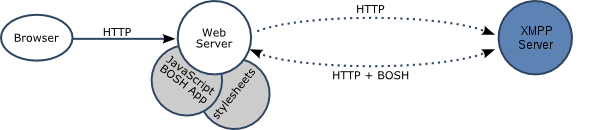
\includegraphics[scale=0.6]{images/xmpp-bosh.png}   
  \caption[BOSH]{XMPP BOSH}
  \label{img:xmpp-bosh}                        
  \end{figure} 

Aside from the socket needed for XMPP communication, each managed connection has two other pieces of data associated with it: the session identifier(SID) and the request identifier(RID). SID stands for Session Identifier. This uniquely identifies the managed XMPP connection, and it is often a long, opaque alphanumeric string. Even though it is enough to identify the session, it is not very useful on its own. The RID identifies a particular HTTP request associated with a BOSH-managed connection. Before a connection is established, the client sends a random RID to the DataStream Manager along with its first request. Each subsequent request increments the RID by one. The SID and the RID together provide enough information to interact with the underlying XMPP connection. Because the RID is generated randomly from a very large range of numbers, it is virtually impossible to guess the RID. Also, the DataStream Manager will reject RIDs that fall outside of a narrow window around the current request. In this way, the BOSH-managed connection is tolerant of small errors like out of order delivery but robust to attacks like hijacking the connection. Because these two identifiers are enough to both address and make use of a managed XMPP session, if an application knows the SID and the RID, it can take over or attach to the underlying session.

The attach() function demonstrats sending SID and RID through a BOSH connection in the Listing~\ref{BOSH_callback}):
	    \begin{lstlisting}[label=BOSH_callback,caption=BOSH Callback]
		var connection = new Strophe.Connection(BOSH_URL);
        connection.attach(jid, sid, rid, callback);
	    \end{lstlisting}

BOSH sessions can be encrypted, and often the underlying XMPP sessions are encrypted as well. Because XMPP makes use of SASL, the authentication mechanisms are strong.

\subsubsection{Message Handler}
In order to support both MUC and PubSub message broadcasting, \verb|XMPP| service in frontend has a set of abstract methods like \verb|subscribe|, \verb|unsubscribe|, \verb|check node| and \verb|handle_message| that work with abstract entities omitting extension protocol details. It also has final methods \verb|handle_incoming_muc| and \verb|handle_incoming_pubsub|, implementing message consuming logic specific to each protocol.

Listing \ref{code:handle_muc} shows simplified implementation of MUC-handler.

\begin{lstlisting}[language=java,label=code:handle_muc,caption=Simplified MUC handler]
	handle_incoming_muc: function (message) {
            var sensor = xmpp.find_sensor(message);
            if (!(sensor)) {
                return true;
            }
            var text = Strophe.getText(message.getElementsByTagName("body")[0]);
            if (sensor.type == 'text') {
              if (typeof text == "string") {
                   Text.updateTextBlock(text, sensor["id"]);
               } else {
                  throw_error("Message is not a Text");
               }
            } else if (sensor.type == 'chart') {
                try {
                    var data_array = JSON.parse(text);
                    }
                } catch (e) {
                    throw_error("message is not a valid JSON", text);
                    return true;
                }
                if (Array.isArray(data_array)) {
                    Graph.update(data_array, sensor.id);
                } else {
                  throw_error("Message is not a JSON array");
               }
            }
            return true;
        },
\end{lstlisting}

%Following points describe the process of handling new incoming message by DataStream Manager



\subsection{User Private Storage}
    \label{xep0049}
	Since web-based application has no access to the local storage of a device and frontend should not directly rely on a database used on the Data Hub, it was decided to use one of the XMPP extensions. Private XML Storage\footnote{XEP0049 specification,\url{http://xmpp.org/extensions/xep-0049.html}} is such an extension, allowing a client to store any arbitrary XML on the XMPP server by sending an \verb|<iq/>| stanza of type ``set'' to the server with a \verb|<query/>| child scoped by the ``jabber:iq:private'' namespace. The purpose of using it is to make a storage for user personal preferences like subscriptions, favorites, accepted SLAs etc.

    The \verb|<query/>| element may contain any arbitrary XML fragment as long as the root element of that fragment is scoped by its own namespace. The data can then be retrieved by sending an \verb|<iq/>| stanza of type ``get'' with a \verb|<query/>| child scoped by the \verb|jabber:iq:private| namespace, which in turn contains a child element scoped by the namespace used for storage of that fragment. Using this method, Jabber entities can store private data on the server and retrieve it whenever necessary. The data stored might be anything, as long as it is a valid XML. One typical usage for this namespace is the server-side storage of client-specific preferences. All available methods are displayed in table~\ref{img:xep49-methods}.
	
	\begin{figure}[!ht]
		\centering
		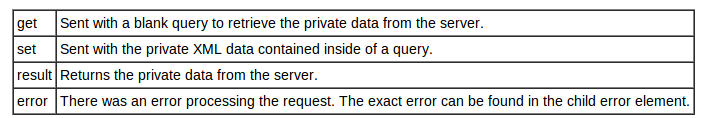
\includegraphics[scale=0.9]{images/xep0049Queries.png}   
		\caption[ Description of Acceptable Methods]{Description of Acceptable Methods}
		\label{img:xep49-methods}
		\end{figure}
	\subsubsection{Elements}
	The root element of Private XML Storage namespace is query. At least one child element with a proper namespace must be included; otherwise the server must respond with a ``Not Acceptable'' error. A client must not query for more than one namespace in a single IQ get request. However, an IQ set or result may contain multiple elements qualified by the same namespace. Examples of saving and loading data are shown on the Listing~\ref{code:client_save} and ~\ref{code:client_load}.

    \begin{lstlisting}[label=code:client_save,caption=Client Stores Private Data]
		CLIENT:
		<iq type="set" id="1001">
		  <query xmlns="jabber:iq:private">
		    <exodus xmlns="exodus:prefs">
		      <defaultnick>Alice</defaultnick>
		    </exodus>
		  </query>
		</iq>

		SERVER:
		<iq type="result" from="alice@likepro.co/"
		    to="alice@likepro.co/" id="1001"/>
    \end{lstlisting}

     \begin{lstlisting}[label=code:client_load,caption=Client Retrieves Private Data]
		CLIENT:
		<iq type="get" id="1001">
		  <query xmlns="jabber:iq:private">
		    <exodus xmlns="exodus:prefs"/>
		  </query>
		</iq>

		SERVER:
		<iq type="result" from="alice@likepro.co/"
		    to="alice@likepro.co/" id="1001">
		  <query xmlns="jabber:iq:private">
		    <exodus xmlns="exodus:prefs">
		      <defaultnick>Alice</defaultnick>
		    </exodus>
		  </query>
		</iq>
    \end{lstlisting}

    The message of format described above can be issued by using two main functions: save (for saving data on the XMPP server) and load (to retrieve saved data from the XMPP server), as shown on the listing~\ref{code:save_load_ns}. Both methods accept an arbitary string as a property key. The method init() initiates creation of registries, subscriptions, favorites and profile storages for a user with empty profile. An example of subscriptons map and favorites array are presented in the Appendix B. All the subsequent manipulations made by a user will be automatically saved and the GUI will be updated automatically by invoking the method reload().
	\begin{lstlisting}[label=code:save_load_ns,caption=Snippet of Save/Load preferences to a private namespace]
	    sensdash_services.factory("User", ["XMPP", "$rootScope", function (xmpp, $rootScope) {
        var user = {
            init: function () {
                user.registries = [];
                user.favorites = [];
                user.subscriptions = {};
                user.profile = {};
            },
            save: function (property) {
                xmpp.connection.private.set(property, property + ":ns", user[property], function (data) {
                        console.log(property + " saved: ", data);
                    },
                    console.log);
            },
            load: function (property) {
                xmpp.connection.private.get(property, property + ":ns", function (data) {
                        user[property] = data != undefined ? data : [];
                        $rootScope.$apply();
                    },
                    console.log);
            },
            reload: function () {
                user.load("registries");
                user.load("profile");
                user.load("subscriptions");
                user.load("favorites");
            }
	\end{lstlisting}

%\subsection{Web Interface Implementation}
%%%%%%%%%%%%%%%%%%%%%%%%%%%%%%%%%%%%%%%%%EVALUATION%%%%%%%%%%%%%%%%%%%%%%%%%%%%%%%%%%%%%%%%%%%%%%%%%%%%%%%%%%%%%%%%%%%%
\section{Evaluation}
Evaluation is done as a proof of concept by demonstrating a use case scenario of an XMPP-driven web dashboard, which retrieves data from a hardware and software sensors. As an example of software sensor a bot was chosen, periodically sending IT news in text format. As a hardware sensor a university temperature sensor was used. Both of them are accessable from respective XMPP chat rooms. A prototype was given a name ``SensDash'' (Sensor Dashboard).

Temperature sensor was provided as a testing environment in scope of ACDSense project, together with TU Dresden, BTU Cottbus - Senftenberg and RWTH Aachen University. It locates in the room INF3086, Faculty of Computer Science, Chair of Computer Science. It represents a class of low-cost, high-performance sensors, which is implemented using a commercially available Raspberry Pi single-board computer with an affiliated USB thermometer and automatic WLAN and XMPP connections to a sensor MUC room established at a boot time. Everything concerning sensors was installed on Mobilis server. According to the system architecture on the Figure \ref{img:system_arch}, everything concerning sensors-side real-time streaming is assumed to be implemented on a DataHub, which includes pre-installed XMPP server supporting BOSH and MUC extensions. The temperature sensor itself is a Data Source 1, and the Data Source 2 is respectively a software sensor presented on the Figure \ref{img:system_arch}.

    \begin{figure}[H]
    \centering
    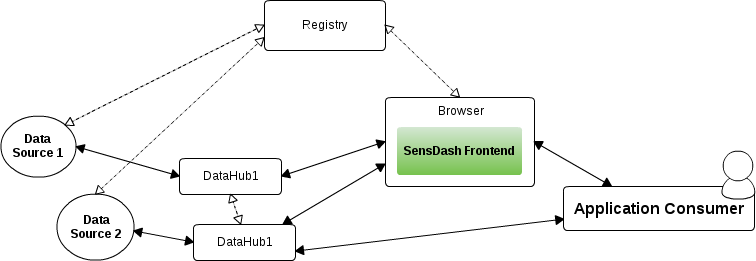
\includegraphics[scale=0.6]{images/UseCaseScheme1.png}   
    \caption[Use Case System Architecture Scheme]{System Architecture Scheme} 
    \label{img:system_arch}                        
    \end{figure}

The temperature sensor publishes data to a MUC room, which can be accessed by jid\\ \verb|xmpp://inf3084@conference.mobilis-dev.inf.tu-dresden.de| and has the description shown on listing~\ref{json_sensor_1}.

	\begin{lstlisting}[label=json_sensor_1,caption=JSON Description of Temperature Sensor]
{
    "sensormuc": {
        "type": "AMBIENT_TEMPERATURE",
        "format": "short",
        "location": {
            "countryCode": "DE",
            "cityName": "Cottbus",
            "latitude": 51.076834,
            "longitude": 13.772586
        }
    }
}
	\end{lstlisting}

First, every sensor has to be put in the Registry with a unique id and fill-in the attributes defined in JSON Registry standard interface. Since not this Master Thesis nor ACDSense project had a task of building Registry software, metadata of temperature and news sensors was added manually as plaintext JSON stubs. The full example of metadata in the Registry can be found in the Appendix A, and the listing~\ref{sensor_registry} presents an excerpt of its main charactristics.

	\begin{lstlisting}[label=sensor_registry,caption=JSON Description of Sensors]
[
    {
            "id": "30",
            "title": "Ambient Temperature INF3084",
            "availability": true,
            "description": "This sensor provides temperature updates with 5-seconds frequency and represents a class of low-cost high-performance sensors. It is implemented using an available Raspberry Pi single-board computer with an affiliated USB thermometer and automatic WLAN and XMPP connections to a sensor MUC room established at boot time.",
            "sla": "Sensor resolution is 0.5 C, measurements taken every 5 seconds. Uptime 95% from 6:00 till 22:00.",
            "sla_last_update":"1395005996",
            "access": "private",
            "provider_name": "Provider TU Dresden",
            "location": "Cottbus",            
            "type": "chart",
            "end_points": [
                {
                    "type": "muc",
                    "name": "xmpp://inf3084@conference.mobilis-dev.inf.tu-dresden.de",
                    "pwd": null
                },
                {
                    "type": "muc",
                    "name": "xmpp://inf3086@conference.mobilis-dev.inf.tu-dresden.de",
                    "pwd": null
                }

            ]
    },
    {
        "id": "20",
        "title": "IT News Feed",
        "availability": true,
        "last_update": "2014-04-05T11:14:34.000+02:00",
        "description": "Provides up to date news in IT and Telecommunication area together with information about new gadgets.",
        "sla": "",
        "sla_last_update": "",
        "access": "public",
        "provider_name": "Provider TU Dresden",
        "location": "Dresden",
        "type": "text",
        "end_points": [
            {
                "type": "muc",
                "priority": "main",
                "name": "xmpp://testraum@conference.mobilis-dev.inf.tu-dresden.de",
                "pwd": null
            }
        ]        
    }
]
	\end{lstlisting}

Use case scenario is demonstrated from 3rd party user prospective -- a mobile application developer Max. First of all he needs to define to which sensor to subscribe and how to retrieve real-time streaming from it. 

\subsection{Use Case Scenario}
\label{section:use-case-scenario}
\textbf{Step 1:} In order to find necessary sensor, description and data format provided by it, Max has to log in into the SensDash by using peronal JID(max\_sensdash@likepro.co) and password, received from an administrator of a SensDash(Fig. \ref{img:log_in}) or auto-created by XMPP registration software.

\begin{figure}[!ht]
\centering
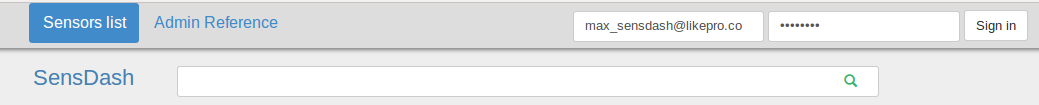
\includegraphics[scale=0.5]{Screenshots/signIn.png}   
\caption[Log in to the SensDash]{Log in to the SensDash}
\label{img:log_in}                        
\end{figure}

\textbf{Step 2:} After successfully completing the authentification process, Max can start browsing, searching and filtering sensors, as shown on the Figure~\ref{img:welcome_screen}.

\begin{figure}[!ht]
\centering
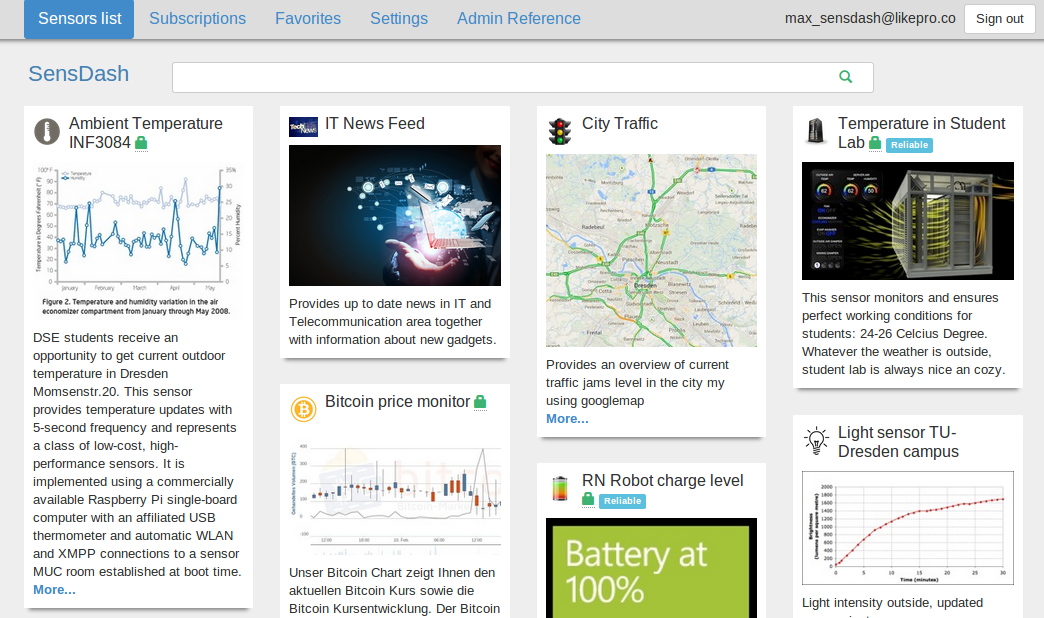
\includegraphics[scale=0.5]{Screenshots/Welcome.png}   
\caption[List of available sensors]{List of available sensors}
\label{img:welcome_screen}                       
\end{figure}

 By using a search field, he can enter keywords that define purpose or type of a sensor, and a list of sensors will be sorted immediately based on the search input. To get more detailed information about sensor user clicks on the sensor box. In a new modal window (Figure ~\ref{img:modal}) user can get a detailed description about sensor, e.g. : SLA, location, provider, preview, development details such as end-points quantity, administrator name and more sophisticated dasription data if required. This information gives an overview of what type of data is provided by data source and which SLA should be accepted if the user wants to subscribe to it.

\begin{figure}[!ht]
\centering
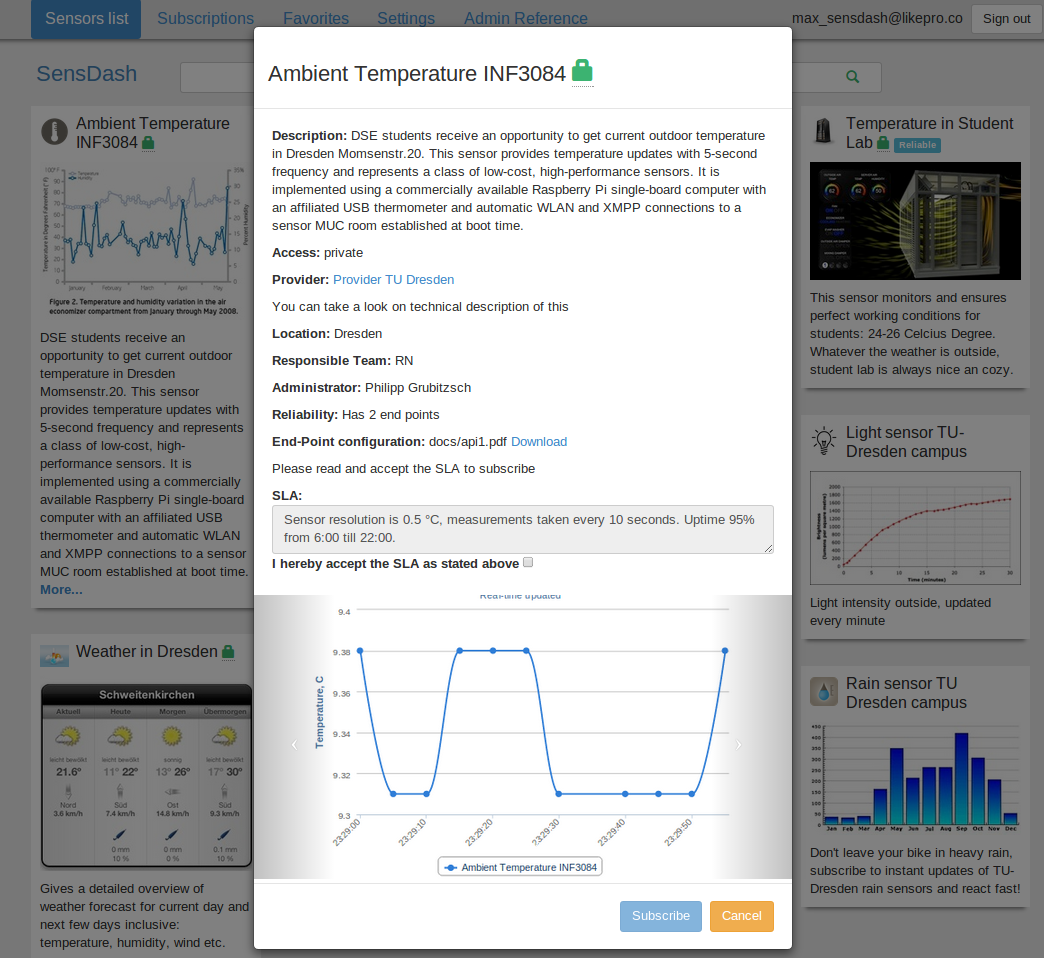
\includegraphics[scale=0.5]{Screenshots/UseCaseWelcome.png}   
\caption[Personal Modal of a Sensor]{Personal Modal of a Sensor}
\label{img:modal}                       
\end{figure}
 
 In case of ambient temperature in room INF3084, Max can explore a predefined preview, which contains graphs of data, its frequency, security level and relialability. In case of software sensor it can be sample of a news feed, provided by sensor. 

\begin{figure}[!ht]
\centering
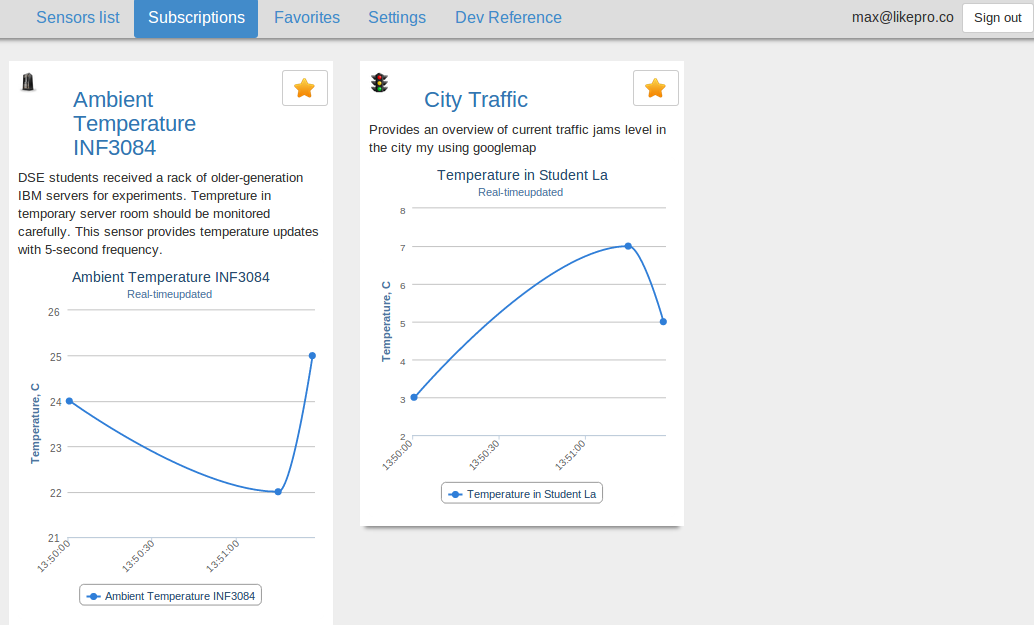
\includegraphics[scale=0.5]{Screenshots/UseCaseScreenshot4.png}   
\caption[Personal Subscribed Sensor]{Subscriptions list} 
\label{img:subscriptions}                        
\end{figure}

\textbf{Step 3:} Since the temperature sensor is a private sensor, Max has to accept SLA before getting a real-time data from it. In contrast with temperature sensor, a software sensor -- IT news feed has a public access, thus, no need to accept any SLA in order to see real-time data provided by this sensor. The common approach, which is applied to every sensor independently from its access type (public or private) is to subscribe to it if desired conditions are met.

This way, all sensors that Max has subscribed to will appear in the next tab called ``Subscriptions''. First, desired amount of history data will be loaded. Then, as soon as new data becomes available SensDash retrieves it (Figure~\ref{img:subscriptions}). By using Subscriptions Tab and icon ``star'' located in a right upper corner, user can add most relevant subscriptions to Favorites. After clicking on the favorites ison, sensors information will appear in the Favorites Tab.

\textbf{Step 4:} To get information about personal account user should navigate to Settings tab. He can find personal profile settings there, as shown on the Figure~\ref{img:settings}.

\begin{figure}[!ht]
\centering
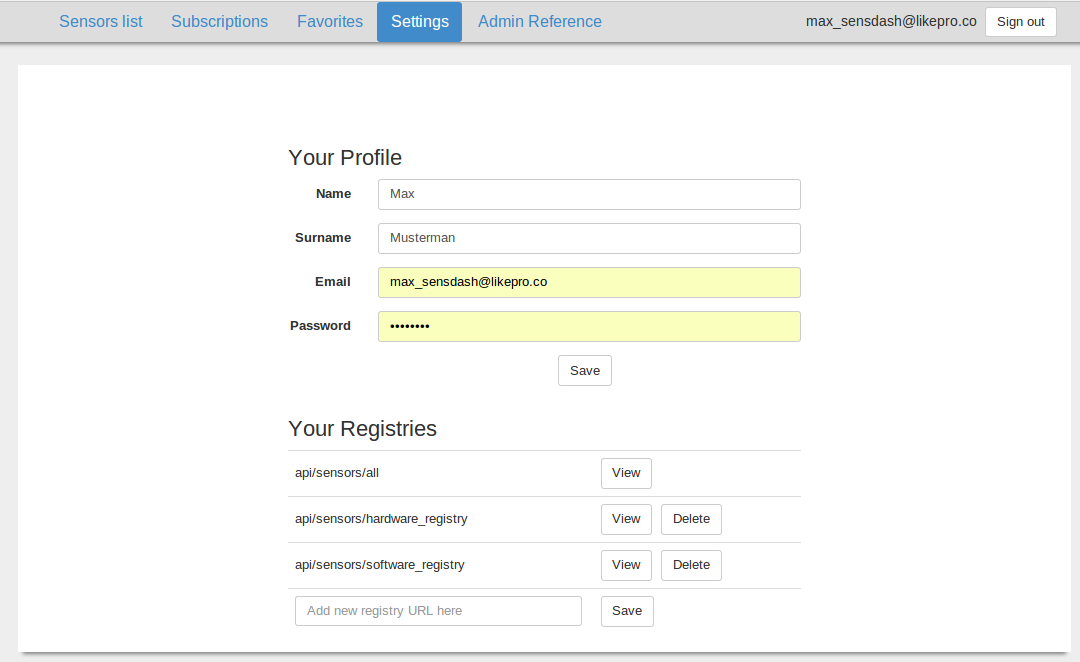
\includegraphics[scale=0.5]{Screenshots/UseCaseScreenshot6.png}   
\caption[Settings Tab]{Settings Tab}
\label{img:settings}                         
\end{figure}

\textbf{Step 5:} As a developer, Max might be interested in technical details of a sensor data retieval process, e.g. API references, end-point configuration, sensor data format and system architecture in order to connect with backend directly or to add a new Registry URL. So Max should navigate to the Admin References Tab (Fig.~\ref{img:admin}), where he can find all available implementation detailes of a SensDash, e.g. used XMPP services and extensions, interface workflow etc. 

\begin{figure}[!ht]
\centering
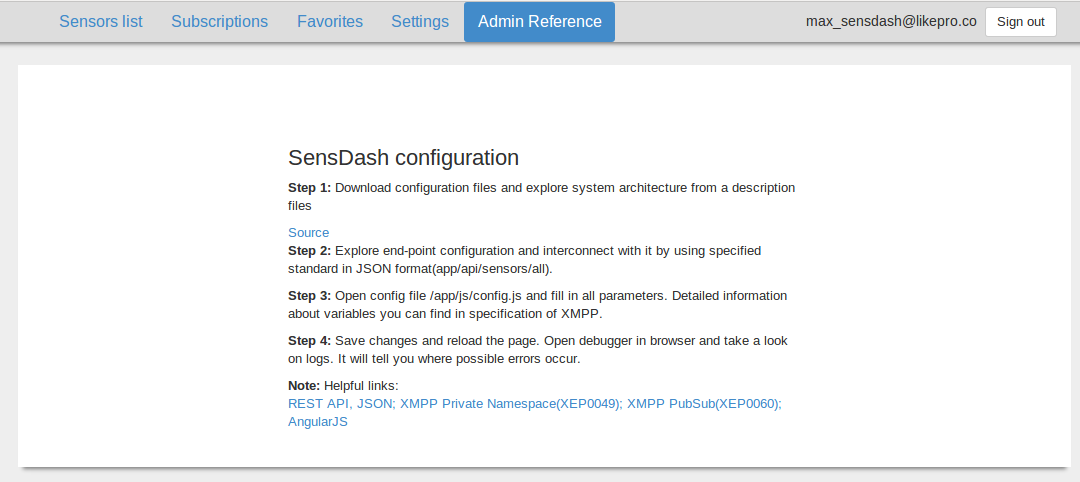
\includegraphics[scale=0.5]{Screenshots/UseCaseReferences.png}   
\caption[Administrator Tab]{Administrator Tab}
\label{img:admin}                         
\end{figure}

\subsection{SensDash Implementation}
Next, SensDash prototype implementation details will be revealed, along with description of main functional modules and XMPP data stream integration.

\textbf{Log In} to the system is allowed only with valid JID and password, registered within XMPP servers. Since XMPP network is highly distributed, it does not metter where exactly the JID belongs to, as long as appropriate permissions are granted within sensor rooms. However, it is important to be aware which XMPP server should carry MUC  room and be responsible for managing real-time data of a sensor.

First, user credentials are checked with regular expression on the frontend side, and than sent to XMPP server. Once XMPP server authenticates the user, a session is saved in the browser using cookies. Next time when the user will open a SensDash, session from cookies will automatically log him/her into the system. 

\textbf{Preferences Persistance} is implemented using XEP0049 and stored on the XMPP server (implementation details available in section~\ref{xep0049}). When a user signs in to the system for the first time, the application logic creates an empty account and initiates empty containers for subscriptions and favorites. Once a user subscribes to any resource, this resource automatically appears in Subscriptions Tab and added to the subscriptions map, saved on the XMPP server. The same is valid for favorites and Favorites Tab. Next time when the user will log in to SensDash, all saved subscriptions, favorites and other private data will be automatically loaded and appear in corresponding tabs. Examples od subscriptions map and favorites array for Max are presented in the Appendix B.

\textbf{SLA Updates}. A hardware or software sensor may have an owner, vendor or provider with whom a user has to sign a service-level agreement (SLA). The Frontend is responsible for retrieving SLA description and its ``last time update'' for the user. Once user has accepted the sensor's SLA, he will receive a real-time data till the moment when SLA will be changed by provider. As soon as SLA ``last time update'' in the list of subscribtions of user will no longer match the SLA ``last time update'' provided by the Registry through the Web API, user will be automatically unsubscribed from corresponding sensor and notified via popup alert window.

\textbf{Search Bar} was made by using frontend-based model filtering, implemented with Angular.js filter concept and directly binded to template. It performs real-time sorting and filtering based on metadata of sensors in all registries. It is fast very straightforward for end-user. 

\textbf{Data Streaming} is the point where Data Hub joins the system as a part of backend. All data streaming works through XMPP extensions. In presented example with ambient temprature in INF3084 a MUC extension (XEP0045) was used for retrieving real-time data through BOSH service. But since generic frontend should support maximum of approaches, PubSub extension (XEP0060) support was also provided. Strophe.js was used as a client-side XMPP library; some code was refactored to be MVC-structured.

SensDash logic was built using AngularJS MVC skeleton (Appendix D). This enabled two-way data binding between controllers and templates, presenting updates from data stream in real-time. Multiple endpoints in sensor metadata provide a ground for building redundant data streams, which have been used for adding an extra layer of reliability and/or security. 

Incoming messages are dispatched to appropriate handlers based on sensor type and ID, this data is cached in a hashmap for instant propagation of updates. Message handler services have been implemented with an aim to be easily pluggable, so that generic frontend can be easily extended with new types of sensors.

\subsubsection{Functional characteristics of a sensor}
In the Section 4.4 3 main functional characteristics were clarified, that grant sensor with properties based on a system architecture.
Since XMPP server was introduced as an essential part of the Data Hub, XMPP MUC rooms have been used as one of possible realization of end-points (Fig.~\ref{img:reliability}). 
\begin{figure}[!ht]
\centering
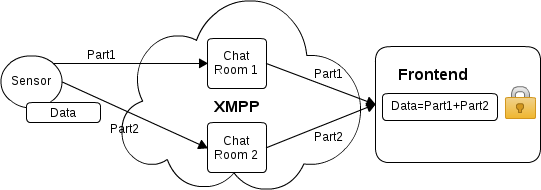
\includegraphics[scale=0.6]{images/security.png}   
\caption[Security]{Data secure transfer using Chat Rooms} 
\label{img:reliability}                        
\end{figure}
Application logic automatically calculates a number of available end-points for every sensor, based on Registry metadata and shows it on the main page, as shown on Figure~\ref{img:icons}. The rules of how the reliability level was calculated is described in the Section 4.4, Subsection ``Sensor Functional Characteristics'' (Appendix C).
\newline
\begin{figure}[!ht]
\centering
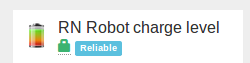
\includegraphics[scale=1.0]{Screenshots/Icons.png}   
\caption[GUI identification of security and reliability level]{GUI identification of security and reliability level}
\label{img:icons}    
\end{figure}


\section{Summary}
This chapter presents implementation details of the generic frontend concept and proposes first working prototype, which is shown by using convincing scenario in the Evaluation section 5.3. The use case was based on subscribing to ambient temperature sensor from the room INF3084 (hardware sensor) and IT news Feed (software sensor).

At the begining of the chapter, development tools, dependencies and environment were discovered and presented: JavaScript and its jQuery extensions as a programming language, AngularJS together with Bootstrap to bind application logic with UI, and Strophe.js -- to implement the XMPP interface and its extensions. Web API interface was defined used to retrieve available sensors metadata from Registries by sending an HTTP GET request to each. Authentification, private data persistance and sensor data stream handling was implemented by using XMPP BOSH protocol, XEP0049 and XEP0045 extensions, using Strophe.js library. In order to connect, disconnet, authorize, save, load, initiate connection through XMPP all these methods and functions were declared based on AngularJS directives, services and controllers.

All used technologies, protocols, libraries and methodologies were gathered in order to implement a working prototype. A summary overview of all mentioned components and tools are shown on the Figure~\ref{img:summary}.

\begin{figure}[H]
\centering
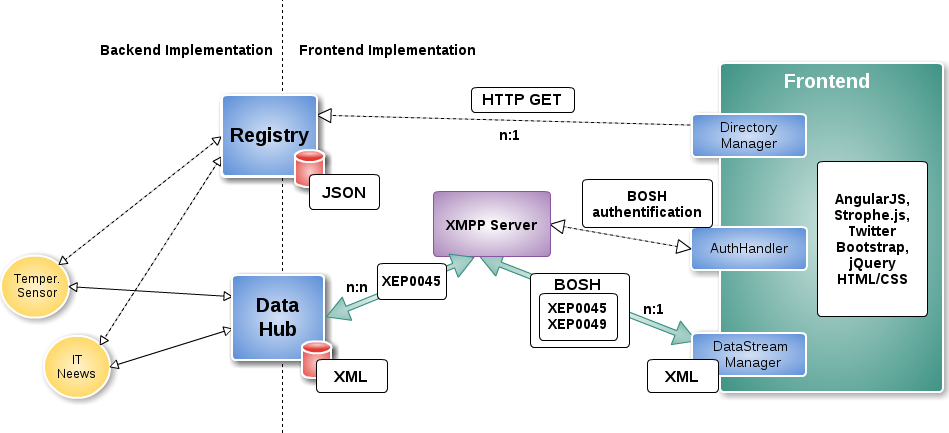
\includegraphics[scale=0.5]{images/ch5Summary.png}   
\caption[Implementation Architecture]{Integrated Implementation Architecture}  
\label{img:summary}                       
\end{figure}

